\documentclass [a4paper, 11pt] {article}
\setlength\parindent{0pt}


\usepackage{amsmath}

\usepackage{blindtext}
\usepackage{graphicx}

% bibliography
\usepackage [style=bwl-FU, url=false, eprint=false]{biblatex}
\addbibresource{biblio.bib}

\setcounter{secnumdepth}{0}


\begin{document}
% title description 
\title {\Huge Final Project \\
 \Huge Digital Tools for Finance }
\author {\huge Elena Ten 19-765-395, \\
	 	 \huge Elena Grigorenko 19-738-343}

\date {\huge 10.12.2020}



% create title
\maketitle
\thispagestyle{empty}

\newpage

\tableofcontents

\newpage

\section {Introduction}
This report is aimed on the estimation of the cost of capital of the main players of the oil industry.\\
The first part of the report gives a brief overview of main market characteristics of oil stocks.\\
The second part of the report is dedicated to the estimation of the cost of capital.

\section {Overview of Market Data}

\section {Cost of Capital}
\subsection {Methodology}

According to \cite{DamodaranDark} and \cite{BestPract}, one of the most prominents methods in calculating the cost of equity is the CAPM model, that is being implemented in the current research.

\subsection {Risk-free rate}

For the estimation of risk-free rates we considered global risk-free rates (Figure ~\ref{fig:rf})

% insert beta plot
\begin{figure}[!h]
\caption{Global risk free rates}
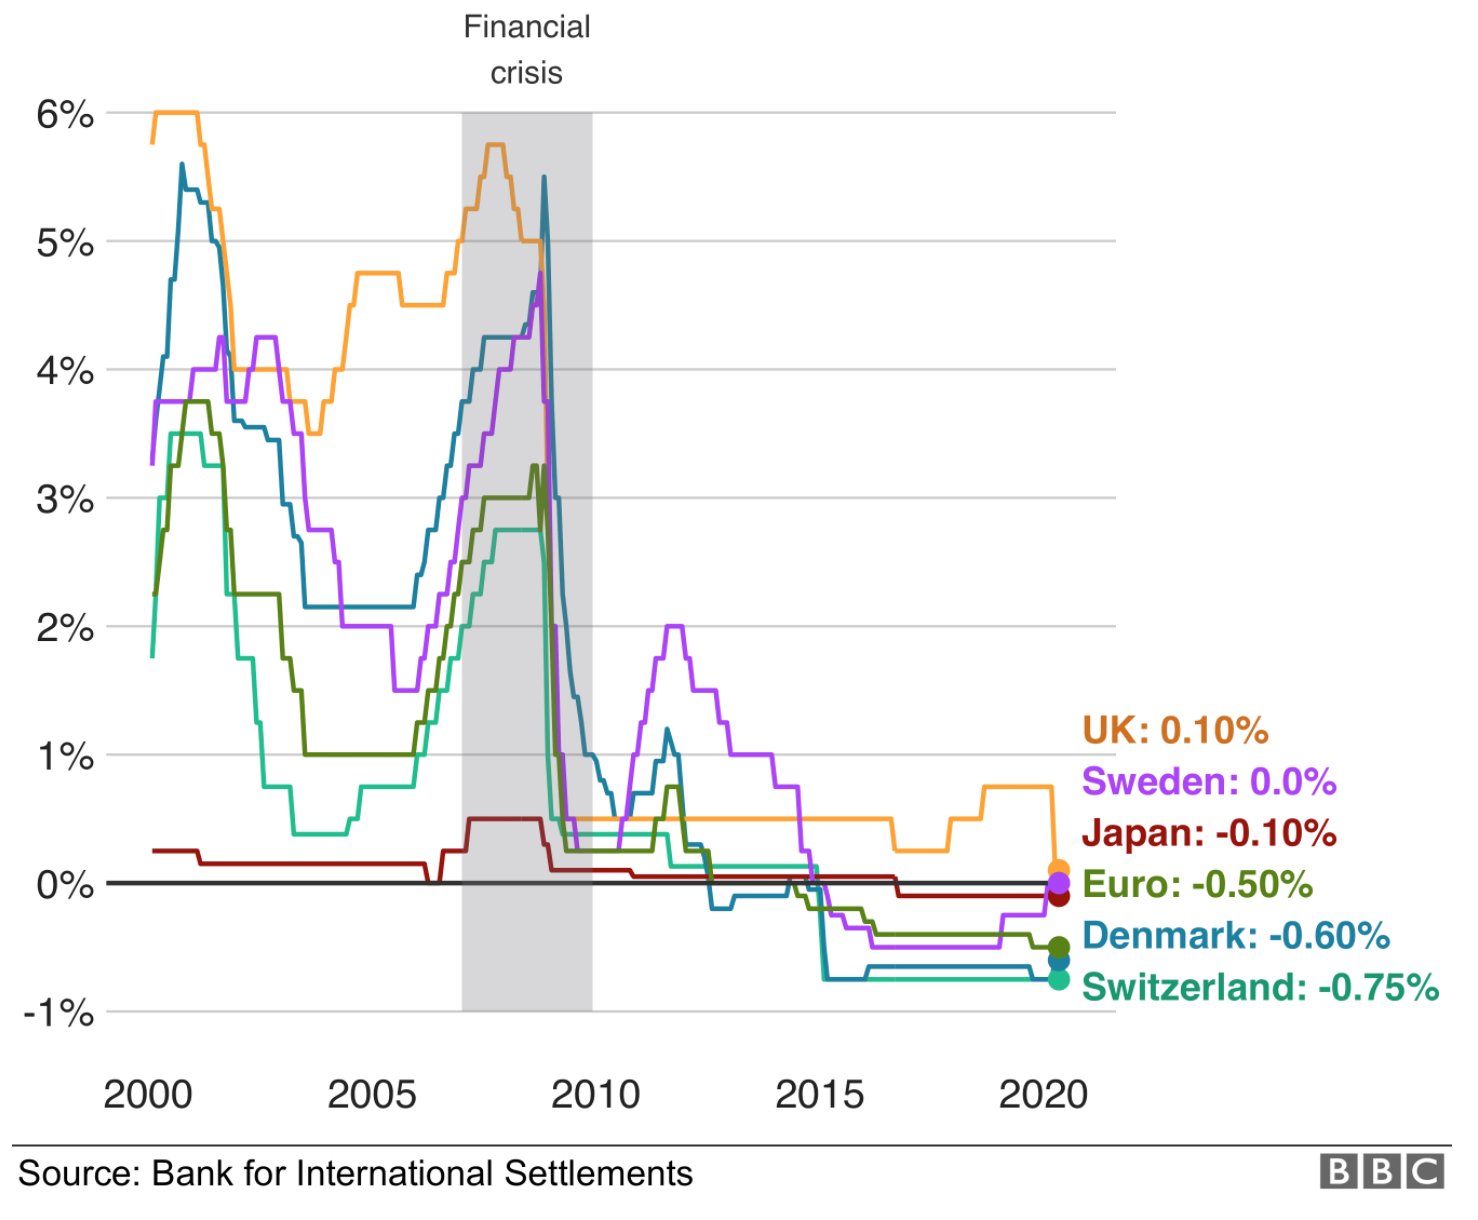
\includegraphics[scale=0.25]{risk_free}
\label{fig:rf}
\end{figure}


The risk free rate for the current project was accepted to be 0.

\subsection {Beta estimation}

Companies' beta coefficients were calculated, using the methodology, described by \cite{DamodaranDark}.\\
The 5 year time period was used for the estimation. The market index was represented by S\&P 500.\\
The results are presented in Table \ref{tab:beta}.\\

% insert beta table 
\begin{table}[!h]
\caption{Beta coefficients\label{beta}} 
\begin{center}
\begin{tabular}{llr}
\hline\hline
%\multicolumn{1}{l}{beta}&\multicolumn{1}{c}{comp_names}&\multicolumn{1}{c}{beta}\tabularnewline
\hline
1&China Petroleum \& Chemical&$0.83$\tabularnewline
2&PetroChina&$0.97$\tabularnewline
3&Royal Dutch Shell PLC&$1.11$\tabularnewline
4&BP PLC&$1.09$\tabularnewline
5&Exxon Mobil Corp.&$1.02$\tabularnewline
6&Total SE&$1.07$\tabularnewline
7&Chevron Corp.&$1.20$\tabularnewline
8&Marathon Petroleum Corp.&$1.54$\tabularnewline
9&PJSC Lukoil&$0.97$\tabularnewline
\hline
\end{tabular}\end{center}
\label{tab:beta}
\end{table}

% insert beta plot
\begin{figure}[!h]
\caption{Beta Coefficients}
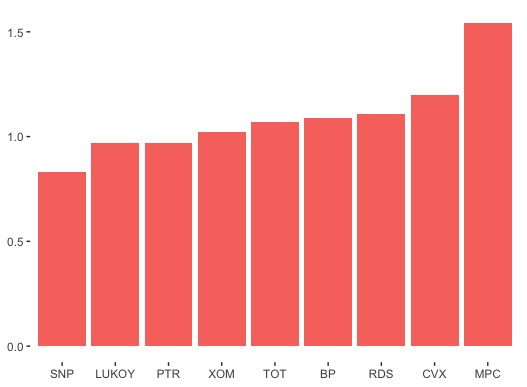
\includegraphics[scale=0.65]{beta_plot_bars}
\label{fig:beta}
\end{figure}


\subsection {Cost of Equity}

Cost of equity was calculated with the CAPM method, ising the following formula:

$$ r_e = r_f + \beta (r_m - r_f)$$

The results of calculations are provided in Table \ref{tab:r_e}.

% insert r_e table
\begin{table}[!h]
\caption{Cost of Capital\label{r}} 
\begin{center}
\begin{tabular}{llr}
\hline\hline
%\multicolumn{1}{l}{r}&\multicolumn{1}{c}{comp_names}&\multicolumn{1}{c}{round.beta_df.beta...r_m..2.}\tabularnewline
\hline
1&China Petroleum \& Chemical&$0.15$\tabularnewline
2&PetroChina&$0.17$\tabularnewline
3&Royal Dutch Shell PLC&$0.20$\tabularnewline
4&BP PLC&$0.19$\tabularnewline
5&Exxon Mobil Corp.&$0.18$\tabularnewline
6&Total SE&$0.19$\tabularnewline
7&Chevron Corp.&$0.21$\tabularnewline
8&Marathon Petroleum Corp.&$0.27$\tabularnewline
9&PJSC Lukoil&$0.17$\tabularnewline
\hline
\end{tabular}\end{center}
\label{tab:r_e}
\end{table}



\subsection {Findings and Conclusion}


\newpage
\printbibliography [heading=bibintoc]

\end{document}
